\documentclass{article}
\usepackage[T1]{fontenc}
\usepackage{lmodern}
\usepackage{graphicx}
\usepackage{amsmath,amssymb}
\usepackage[a4paper,margin=2cm]{geometry}
\usepackage[absolute,overlay]{textpos}
\setlength{\TPHorizModule}{1mm}
\setlength{\TPVertModule}{1mm}
\usepackage[indonesian]{babel}
\usepackage{hyperref}
\setlength{\emergencystretch}{2em}
% unit: Halaman 26

\begin{document}

% === Halaman 26 (llm) ===

\vspace{100.98mm}

\section*{Inversi Permutasi ($\text{IP}^{-1}$)}

\begin{itemize}
    \item Permutasi terakhir dilakukan setelah 16 kali putaran terhadap gabungan blok kiri dan blok kanan.
    \item Permutasi menggunakan matriks permutasi awal balikan ($\text{IP}^{-1}$) sbb:
\end{itemize}

\vspace{10mm}

\begin{tabular}{|c|c|c|c|c|c|c|c|c|c|c|c|c|c|c|c|}
\hline
40 & 8 & 48 & 16 & 56 & 24 & 64 & 32 & 39 & 7 & 47 & 15 & 55 & 23 & 63 & 31 \\ \hline
38 & 6 & 46 & 14 & 54 & 22 & 62 & 30 & 37 & 5 & 45 & 13 & 53 & 21 & 61 & 29 \\ \hline
36 & 4 & 44 & 12 & 52 & 20 & 60 & 28 & 35 & 3 & 43 & 11 & 51 & 19 & 59 & 27 \\ \hline
34 & 2 & 42 & 10 & 50 & 18 & 58 & 26 & 33 & 1 & 41 & 9 & 49 & 17 & 57 & 25 \\ \hline
\end{tabular}

% deskripsi: Diagram alur proses enkripsi DES yang menunjukkan langkah-langkah dari blok plaintext, Initial Permutation (IP), 16 kali putaran Enciphering dengan Key expansion, hingga Inverse Initial Permutation (IP-1) untuk menghasilkan blok ciphertext.
% bbox normalisasi: [0.7100, 0.0000, 0.9900, 0.3400]
\begin{textblock*}{58.80mm}(149.10mm,0.00mm)
\noindent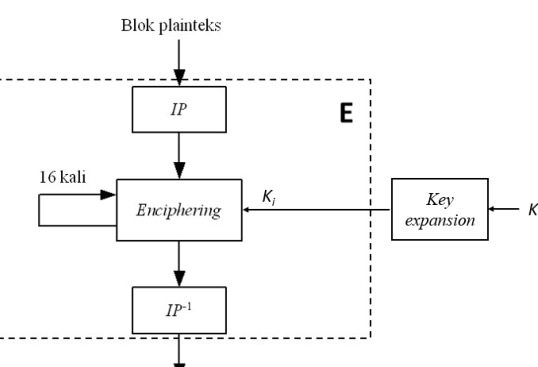
\includegraphics[width=58.80mm,height=100.98mm]{../../images/llm/page_026_img_01.png}%
\end{textblock*}

\end{document}
